\chapter{Programowanie i konfiguracja modułu}
Aspekty programistyczne takie jak wybór środowiska, języka programowania, nazewnictwo zmiennych, koncepcja programowania Arduino oraz działanie przerwań zostały wyjaśnione poniżej. W kolejnej części rozdziału pokazane zostały konkretne implementacje kodowe obsługi poszczególnych modułów wraz z listingami kodu.

\section{Schemat ideowy}
Główna koncepcja programu polega na przetwarzaniu danych wejściowych przez moduł, który wykonuje obliczenia co określoną ilość czasu. Następnym krokiem jest obrobienie oraz wyświetlenie danych. Na rys.~\ref{fig:schemat} przedstawiono ideową koncepcję działania programu w formie schematu.

\begin{figure}[!htb]
\centering
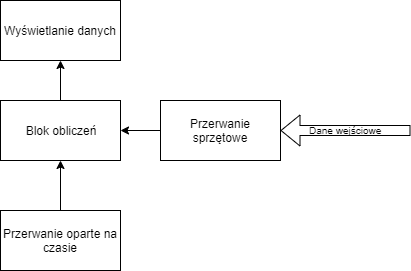
\includegraphics[width=0.7\linewidth]{Rysunki/schemat_logiczny.png}
\caption{Schemat logiczny systemu}
\label{fig:schemat}
\end{figure}

\section{Środowisko programistyczne}

Domyślnym środowiskiem programistycznym (IDE) jakie udostępnia Arduino jest \texttt{Arduino} IDE i to właśnie w nim tworzony oraz kompilowany został kod źródłowy mikrokontrolera. Wybór IDE argumentuję tym, iż posiada ono największe wsparcie ze strony producenta modułu oraz społeczności. Nie ma również zbyt wielu alternatyw. Językiem programowania jakie wpiera Arduino jest \texttt{C}, dlatego też został on użyty do zaprogramowania modułu.

\subsubsection{Przyjęte nazewnictwo podczas pisania kodu}
W obrębie projektu zostało postanowione, że nazwy zmiennych będą zapisywane w języku polskim. Zwykłe zmienne będą nazywane w konwencji \texttt{snake\_case} a nazwy funkcji w \texttt{camelCase}. Dodatkowo wprowadzono znacznik ---, który oznacza, że w tym miejscu znajduje się jakiś kod, jednak jest on pominięty w listingu, ponieważ nie wnosi nic do aktualnego przykładu.

\subsubsection{Koncepcja programowania modułu Arduino}
Strukturę kodu źródłowego można podzielić na dwie główne części: blok ustawień (setup) oraz główną pętle programu (loop).
\begin{itemize}
\item{sekcja, a w zasadzie funkcja \texttt{setup()} wykonuje się tylko raz i służy do ustawiania trybów pinów, inicjalizacji zmiennych, importowania bibliotek, ustawiania przerwań itp.}
\item{główna funkcja programu, a konkretniej \texttt{loop()} jest pętlą, która z założenia wykonuje się w nieskończoność, więc to w niej będą wykonywać się obliczenia, wyświetlanie danych itp.}
\end{itemize}

\section{Przerwania}
\subsubsection{Sprzętowe}
Jednym z najważniejszych zagadnień, bez których zbudowanie projektu byłoby znacznie utrudnione, są przerwania. Przerwania są to sygnały, które jak sama nazwa wskazuje powodują przerwanie wykonywania głównej pętli programu i wykonują zadane polecenia. W tym projekcie będą używane dwa przerwania: pierwsze służące do reagowania na sygnał z VSS oraz drugie, które będzie przesyłać informacje o włączeniu/wyłączeniu wtrysku.\\

Piny przerwań są to cyfrowe piny wejściowe, które mogą mieć tylko dwa stany \texttt{LOW} lub \texttt{HIGH}\\

Arduino Leonardo posiada 4 ustawienia przerwań \cite{ard_ref}
\begin{itemize}
    \item \texttt{LOW} - aktywowane jest wtedy, kiedy stan pinu jest LOW,
    \item \texttt{CHANGE} - aktywowane jest wtedy, kiedy stan zmienia się,
    \item \texttt{RISING} - aktywowane jest wtedy, kiedy stan zmienia się z \texttt{LOW} na \texttt{HIGH} 
    \item \texttt{FALLING} - aktywowane jest wtedy, kiedy stan zmienia się z \texttt{HIGH} na \texttt{LOW} 
\end{itemize}

\subsubsection{Oparte na czasie}
Oprócz przerwań opartych na stanach cyfrowych pinów potrzebne jest również przerwanie, które wykonuje się co określony czas, aby móc przetworzyć i wyświetlić informację. Arduino w swojej dokumentacji nie posiada informacji na temat takich przerwań, jednak jako, iż oparte jest ono na architekturze AVR, która takie przerwania posiada, zostaną one wykorzystane \cite{atmega_datasheet}.\\

\section{Implementacja}
\subsection{Przerwanie timera} \label{setting_timer_interupt}

Zostało założone, że częstotliwość obliczania oraz wyświetlania informacji to 1 sekunda. W tym celu zostanie stworzone przerwanie, które będzie się opierać na dość dokładnym pomiarze czasu, który bazuje na ilości taktów procesora.\\

W poniższym listingu został pokazany kod, który korzysta z Timera 1, który wywołuje przerwanie co 1/4 sekundy. Instrukcje, które zostaną wprowadzone w funkcji \texttt{coSekunde()} będą się wykonywać co dokładnie jedną sekundę.

\begin{lstlisting}[label=list:timer_int,caption=Ustawianie przerwania timera,
basicstyle=\footnotesize\ttfamily]
volatile int licznik_przerwania;
---
void coSekunde()
{
    // Instrukjce w tym miejscu będą wykonywane co sekudnę
}

// Przerwanie wykonywane co 1/4 sekundy
ISR(TIMER1_OVF_vect)
{
    licznik_przerwania++;
    TCNT1 = 3036;
    
    if(licznik_przerwania > 3) 
    {
        coSekunde();

        TCNT1 = 3036;
        licznik_przerwania = 0;
    }
}
---
void setup()
{
---
    TCCR1A = 0x00;
    TCNT1 = 3036;
    TCCR1B |= ((1 << CS10) | (1 << CS11));
    TIMSK1 |= (1 << TOIE1);
---
}
---
\end{lstlisting}



\subsection{Aktualna prędkość}
\subsubsection{Konfiguracja przerwania}

Do obliczenia prędkości zostało wykorzystane przerwanie typu FALLING, aby każdy z sygnałów został zliczony.

Jak zostało przestawione w \ref{vss} sygnał od VSS jest podłączony do pinu 7, który obsługuje przerwanie 4.

\begin{lstlisting}[label=list:vss_int,caption=Ustawianie przerwania VSS,
basicstyle=\footnotesize\ttfamily]
volatile int licznik_impulsow;

const vss_pin_int = 4;
---
void liczenieImpulsow()
{
    licznik_impulsow++;
}
---
void setup()
{
---
    attachInterrupt(vss_pin_int, liczenieImpulsow, FALLING);
---
}
---
\end{lstlisting}
\subsubsection{Obliczenia} \label{code_speed}

W celu wyliczenia aktualnej prędkości zostały zastosowane obliczenia z \ref{calc_speed} oraz funkcja \texttt{coSekunde()} z \ref{setting_timer_interupt}.

\begin{lstlisting}[label=list:vss_int,caption=Wyliczanie aktualnej prędkości,
basicstyle=\footnotesize\ttfamily]
volatile int impulsy_vss;
float predkosc;
const float mila = 1.609344;
---
void coSekunde()
{
    predkosc = (mila/4000.0)*impulsy_vss*3600;
    impulsy_vss = 0;
}
---
\end{lstlisting}

\subsection{Aktualne spalanie}
\subsubsection{Konfiguracja przerwania}

Do obliczenia aktualnego spalania zostało wykorzystane przerwanie typu \texttt{CHANGE}. W ten sposób gdy pin zmieni swój stan zostanie mierzony czas otwarcia wtrysku w mikrosekundach

Jak zostało przestawione w \ref{inj} sygnał od wtrysku jest podłączony do pinu 2, który obsługuje przerwanie 1.

\begin{lstlisting}[label=list:inj_int,caption=Ustawianie przerwania wtrysku,
basicstyle=\footnotesize\ttfamily]

volatile unsigned long czas_stanu_low;
volatile unsigned long czas_stanu_high;
volatile unsigned long czas_otwarcia_wtrysku;

const inj_pin = 2;
const inj_pin_int = 1;
---
void liczenieCzasuOtwarciaWtrysku()
{
    if (digitalRead(inj_pin) == LOW)
    {
        czas_stanu_low = micros();
    }
    if (digitalRead(inj_pin) == HIGH)
    {
        czas_statnu_high = micros();
        czas_otwarcia_wtrysku += czas_stanu_high-czas_stanu_low;
    }
}
---
void setup()
{
---
    attachInterrupt(inj_pin_int, liczenieCzasuOtwarciaWtrysku, CHANGE);
---
}
---
\end{lstlisting}

\subsubsection{Obliczenia}

Do wyliczenia aktualnego spalanie zostały zastosowane obliczenia z \ref{calc_consumption}, funkcja \texttt{coSekunde()} z \ref{setting_timer_interupt} oraz obliczona już prędkość z poprzedniego podrozdziału \ref{code_speed}.

\begin{lstlisting}[label=list:vss_int,caption=Obliczanie aktualnego spalania,
basicstyle=\footnotesize\ttfamily]
float predkosc;
float spalanie_s;
float spalanie_h;
float spalanie_100;

const stala_wtrysku = 190;

---
void coGodzine()
{
---
    spalanie = ((stala_wtrysku/60*(czas_otwarcia_wtrysku/1000000.0))*4.0);
    spalanie_h = ((spalanie/1000.0)*3600.0);
    spalanie_100 = ((100*spalanie_h)/predkosc);
---
}


\end{lstlisting}


\subsection{Położenie pedału gazu}

Sygnał położenia pedału gazu działa niczym potencjometr. Do obliczenia jego procentowej wartości została użyta funkcja \texttt{analogRead}, która ma rozdzielczość 10 bit i zwraca liczbę całkowitą z przedziału 0-1023 w zależności od odczytu na wejściu \cite{ard_ref}.

\begin{lstlisting}[label=list:code_thr,caption=Obliczanie procentowego nacisku na pedał gazu,
basicstyle=\footnotesize\ttfamily]

const thr_pin = 0;

---
float aktualnyNacisk()
{
    int odczyt;
    
    // Przeskalowany, ponieważ sygnał nigdy nie równa się 5V
    odczyt = analogRead(thr_pin)-88.0; 
    
     // Zwraca nacisk w procentach
    return odczyt/(1023-88) * 100;
}
---
\end{lstlisting}


\subsection{Odczyt woltomierza} \label{voltometer_code}

Aplikacja ma również informować użytkownika o aktualnym napięciu w układzie samochodu. W tym celu zostały użyte dwa rezystory (\ref{voltometer}).

\begin{lstlisting}[label=list:code_thr,caption=Obliczanie aktualnego napięcia,
basicstyle=\footnotesize\ttfamily]

const voltometer_pin = 1;

float R1 = 100000.0; // Opór rezystora R1
float R2 = 10000.0; // Opór rezystora R2

---
float woltomierz()
{
    int odczyt = analogRead(voltometer_pin);
    float napiecie_na_wyjsciu = (odczyt * 5.0) / 1024.0;
    float wartosc_napiecia = napiecie_na_wyjsciu / (R2/(R1+R2));
    
    // Zabezpieczenie, aby nie wyświetlać pomiaru w granicy błędu
    if (wartosc_napiecia<0.09)
    {
    	return 0.0;
    }
    
    return wartosc_napiecia;
}
---
\end{lstlisting}


\subsection{Mikro przełącznik}

\subsubsection{Ustawianie trybu podciągającego}

Poprawne działanie mikro przełącznika zostało zapewnione dzięki wbudowanemu w Arduino rezystorowi podciągającemu, dzięki któremu nie będzie przypadków, iż na wejściu będzie panował stan nieznany. Arduino Leonardo umożliwia ustawienie pinu w tryb \texttt{PULLUP}, dzięki czemu nie potrzeba dokładać kolejnego rezystora. 
\begin{lstlisting}[label=list:code_pullup,caption=Ustawianie pinu switcha w tryb PULLUP,
basicstyle=\footnotesize\ttfamily]

const switch_pin = 13;

void setup()
{
    pinMode(switch_pin,INPUT_PULLUP);
    digitalWrite(switch_pin, HIGH);
}
---
\end{lstlisting}

\subsubsection{Drgania mikro przełącznika}
Większość mikro przełączników mechanicznych posiada problem z drganiami styków. W przypadku, gdy przycisk zostaje wciśnięty lub puszczony jego styki potrafią drgać powodując zmianę stanu wejściowego na pinie. W celu zabezpieczenia się przed tym została napisana funkcja, która po zmianie stanu na wejściu czeka określoną ilość czasu i sprawdza raz jeszcze stan przycisku, aby uniknąć błędów. Dla tego typu mikro przełączników przyjęło się, iż ten okres czasu wynosi 20 $\mathrm{\mu s}$.\\

Zaimplementowano dwa tryby klikania w mikro przełącznik, aby polepszyć możliwości interakcji z użytkownikiem, są to: zwykłe kliknięcie oraz przytrzymanie (min. 1 sekundę).

\begin{lstlisting}[label=list:code_switch,caption=Obsługa mikroprzełacznika,
basicstyle=\footnotesize\ttfamily]

#define czas_drgan 20
#define czas_przytrzymania 1000

const switch_pin = 13;

int switch_wartosc = 0;
int switch_ostatnia_wartosc = 0;
long czas_przycisku_wcisnietego;
long czas_przycisku_puszczonego;
boolean ignoruj_nacisniecie = false; 


void nacisnieciePrzycisku()
{
    // To wykona się po naciśnięciu przycisku
}
void przytrzymaniePrzycisku()
{
    // To wykona się po przytrzymaniu przycisku
}
void mirkroPrzelacznik()
{

	switch_wartosc = digitalRead(switch_pin);

    if (
        switch_wartosc == LOW && 
        switch_ostatnia_wartosc == HIGH && 
        (millis() - czas_przycisku_puszczonego) > long(czas_drgan)
    )
    {
    	czas_przycisku_wcisnietego = millis();
    }
    
    if (
        switch_wartosc == HIGH &&
        switch_ostatnia_wartosc == LOW &&
        (millis() - czas_przycisku_wcisnietego) > long(czas_drgan))
    {
    	if (ignoruj_nacisniecie == false)
    	{
    		nacisnieciePrzycisku();
    	}
    	else
    	{
    	    ignoruj_nacisniecie = false;
    	}
    	czas_przycisku_puszczonego = millis();
    }
    
    if (
        switch_wartosc == LOW &&
        (millis() - czas_przycisku_wcisnietego) > long(czas_przytrzymania))
    {
    	przytrzymaniePrzycisku();
    
    	ignoruj_nacisniecie = true;
    	czas_przycisku_wcisnietego = millis();
    }
    
    switch_ostatnia_wartosc = switch_wartosc;
}
---
\end{lstlisting}

\subsection{Wyświetlacz LCD}

Ze względu na to, iż wyświetlacz jest zgodny ze sterownikiem HD44780 została użyta biblioteka \texttt{LiquidCrystal.h} \cite{lib_lcd}, która umożliwia łatwą komunikację z kontrolerem sterującym wyświetlaczem.

\begin{lstlisting}[label=list:lcd_setup,caption=Inicjalizacja wyświetlacza,
basicstyle=\footnotesize\ttfamily]
#include <LiquidCrystal.h>
---
void setup()
{
---
    LiquidCrystal lcd(12,11,6,5,4,3);
---
}
---
\end{lstlisting}

\subsection{Czujnik temperatury} \label{one_wire_temp}

Wsparcie dla cyfrowego czujnika temperatury działającego na interfejsie 1-Wire zostało zapewnione dołączając dwie biblioteki: \texttt{DallasTemperature.h} \cite{lib_dallas}, która odpowiada za odczyt i konfiguracje czujnika oraz \texttt{OneWire.h} \cite{lib_onewire}, dzięki której można korzystać z interfejsu 1-Wire.

\begin{lstlisting}[label=list:d18s20_setup,caption=Inicjalizacja czujnika i odczyt temperatury,
basicstyle=\footnotesize\ttfamily]
#include <OneWire.h>
#include <DallasTemperature.h>

#define ONE_WIRE_BUS 10

OneWire oneWire(ONE_WIRE_BUS);
DallasTemperature sensors(&oneWire);

---
void setup()
{
---
    sensors.begin();
---
}

float temperatura() 
{
    sensors.requestTemperatures();
    return sensors.getTempCByIndex(0);
}
---
\end{lstlisting}


\subsection{Pamięć nieulotna EEPROM}
Pamięć EEPROM (ang. Electrucally-Erasable Programmable Read-Only Memory) jest to rodzaj pamięci nieulotnej. Można z niej odczytywać nieograniczoną ilość razy, jednak ilość zapisań/kasowań jest ograniczona. W przypadku Arduino w wersji Leonardo ograniczenie to wynosi 100000 cykli. Wielkość pamięci w tej wersji płytki wynosi 1 kB, przy czym jedna komórka pamięci może mieć wartość od 0 do 255 bitów.\\
W celu zapisywania/odczytywania danych z EEPROM została użyta biblioteka \texttt{EEPROM.h} \cite{lib_eeprom}. Dostarcza ona m.in metody, które umożliwiają zapis tj. \texttt{EEPROM.write()} oraz odczyt tj. \texttt{EEPROM.read()}.
\subsubsection{Operacje na większych danych}
W przypadku tego projektu dane, które są zapisywane to przejechany dystans oraz spalone paliwo. Aby móc zapisać i odczytać tak duże wartości zostały zaimplementowane funkcje \texttt{EEPROMZapiszLong()} oraz \texttt{EEPROMOdczytajLong()}, które umożliwiają zapis 32 bitowego typu \texttt{long} na czterech komórkach pamięci umożliwiających zapis 8 bitowych danych.

\begin{lstlisting}[label=list:eeprom_long,caption=Zapis i odczyt dużych liczb do/z EEPROM,
basicstyle=\footnotesize\ttfamily]
#include <EEPROM.h>
---
void EEPROMZapiszLong(int adres, long wartosc)
{
    byte czwarty = (wartosc & 0xFF);
    byte trzeci = ((wartosc >> 8) & 0xFF);
    byte drugi = ((wartosc >> 16) & 0xFF);
    byte pierwszy = ((wartosc >> 24) & 0xFF);
    
    EEPROM.write(adres, czwarty);
    EEPROM.write(adres + 1, trzeci);
    EEPROM.write(adres + 2, drugi);
    EEPROM.write(adres + 3, pierwszy);
}

long EEPROMOdczytajLong(long adres)
{
    long czwarty = EEPROM.read(adres);
    long trzeci = EEPROM.read(adres + 1);
    long drugi = EEPROM.read(adres + 2);
    long pierwszy = EEPROM.read(adres + 3);
    
    return 
    ((czwarty << 0) & 0xFF)
    + ((trzeci << 8) & 0xFFFF)
    + ((drugi << 16) & 0xFFFFFF) 
    + ((pierwszy << 24) & 0xFFFFFFFF);
}
\end{lstlisting}

Zostało założone, iż ilość spalonego paliwa jest zapisywana od zerowej komórki pamięci, a przejechany dystans od czwartej. To oznacza, że aby odczytać zapisane dane należy wywołać funkcje \texttt{EEPROMOdczytajLong(0)}, aby odczytać spalone paliwo oraz \texttt{EEPROMOdczytajLong(4)}, aby odczytać przejechany dystans. Analogicznie jest z zapisem.

\subsubsection{Ograniczenia i optymalizacja}

Ilość zapisów do pamięci EEPROM jest ograniczona. W celu wydłużenia jej żywotności została wprowadzona optymalizacja zapisu do pamięci. Zapis aktualnych danych jest wykonywany tylko, gdy samochód stoi (czyli prędkość pojazdu jest mniejsza niż 2 km/h) oraz gdy dystans od poprzedniego zapisu jest większy niż kilometr. Takie podejście znacznie zredukowało liczbę zapisów.